\documentclass{article}
\usepackage[utf8]{inputenc}
\usepackage[T1]{fontenc}

\usepackage{fullpage}

\usepackage{tikz}
%\usetikzlibrary{calc,arrows,shapes,backgrounds,patterns,fit,decorations,decorations.pathmorphing}

\usepackage[shadow,colorinlistoftodos,textwidth=2.5cm]{todonotes}
\usepackage[final,colorlinks,hyperindex,unicode=true,pdftitle=SPAdes Manual]{hyperref}
\usepackage{url}
\usepackage{booktabs}

\def\spades{SPAdes}
\def\bh{BayesHammer}
\def\ecoli{\it E.~coli}

\usepackage{textcomp}
\usepackage{listings}
\definecolor{light-gray}{gray}{0.92}
\lstset{
  upquote=true,
  columns=fullflexible,
  basicstyle=\ttfamily,
  framerule=0pt,
  frame=single,
  backgroundcolor=\color{light-gray},
  literate={*}{{\char42}}1
           {-}{{\char45}}1
}

%\usepackage[space=true]{accsupp}
%% requires the latest version of package accsupp
%\newcommand{\copyablespace}{
%    \BeginAccSupp{method=hex,unicode,ActualText=00A0}
%\ %
%    \EndAccSupp{}
%}


%\newenvironment{mycode}
%  {\begin{lstlisting}}
%  {\end{lstlisting}}

\begin{document}
\title{{\spades} 2.0.0 Manual\\{\small 
  Revision: \today}}
\date{}
\maketitle

{\spades} stands for St.~Petersburg genome assembler.
It is intended for both single cell and standard (multicell) 
assemblies. {\spades} comes with error correction tool called 
BayesHammer. This manual will help you to install and run
{\spades}.\todo{Are we going to add SEQuel to our pipeline?}

The latest version of the manual can be downloaded at \url{http://bioinf.spbau.ru/spades}.


\renewcommand{\contentsname}{}
\tableofcontents

%\pagebreak

%\listoftodos

\pagebreak

\section{General setting}
\subsection{Notation}
{\spades} works with single and paired end reads.
The following picture explains the notions of 
read size, distance, gap, and insert length
for paired end reads.

\begin{center}
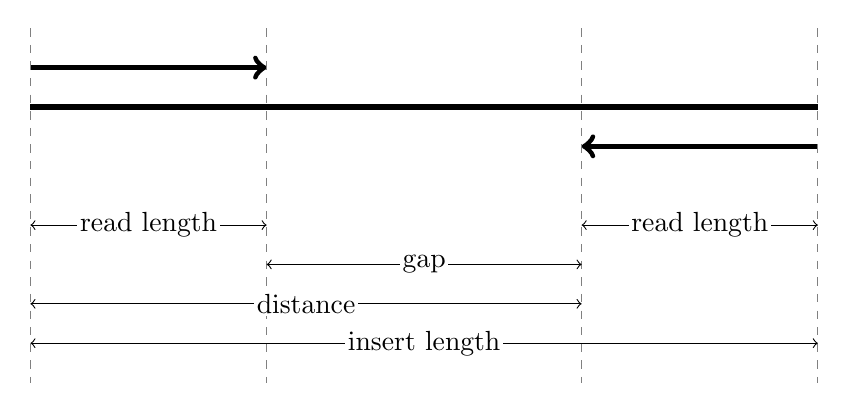
\begin{tikzpicture}
%\draw[help lines] (0,-3) grid (10,3);
\draw[line width=2pt] (0,2) -- (10,2);
\draw[line width=2pt,->] (0,2.5) -- (3,2.5);
\draw[line width=2pt,->] (10,1.5) -- (7,1.5);

\foreach \x in {0, 3, 7, 10}
  \draw[dashed,gray] (\x,3) -- (\x,-1.5);

\foreach \f/\s/\y/\t in {0/3/0.5/read length, 7/10/0.5/read length, 3/7/0/gap, 0/7/-0.5/distance, 0/10/-1/insert length}
\path[<->,draw] (\f,\y) -- node[fill=white,inner sep=1pt,rectangle] {\t} (\s,\y);
\end{tikzpicture}
\end{center}

\subsection{Config files and commands}
Config files and commands are given in gray boxes. 
Note that the text can be copy-pasted directly from this document.
Note also that all the links and all the colored text in the manual are clickable.
In config files, parts of lines starting with a semicolon are just comments.

\section{Requirements}
\subsection{Operating System}
{\spades} requires a 64-bit Linux system.
You need to have root privileges in order to install {\spades}.

\subsection{RAM}
Assembling our test multi-cell {\ecoli} dataset 
by {\spades} uses about 700~Mb peak memory, and single cell
{\ecoli} dataset uses 6~Gb peak memory. 
Correcting errors in these datasets requires about 70~Gb of RAM.
These datasets can be found at \url{http://spades.bioinf.spbau.ru/spades_test_datasets}.

\section{Installing {\spades}}
\todo[inline]{are we going to support manual installation (with installprereqs and so on)?}

\subsection{Installing on Debian-based Linux System}
First add the repository containing {\spades} by inserting the following line
to the file {\tt /etc/apt/sources.list}
\begin{lstlisting}
deb http://debian.bioinf.spbau.ru /
\end{lstlisting}
After that, {\spades} can be installed just by typing
\begin{lstlisting}
sudo apt-get install spades
\end{lstlisting}

\subsection{Installing on ...}
\todo[inline]{what about other types of Linux?}


\subsection{Testing your installation}
To check your installation type
\begin{lstlisting}
spades.py
\end{lstlisting}
This runs {\spades} on a toy dataset (first 1,000 bp of {\ecoli}) that {\spades} comes with. If the installation was successfull you will see the following lines in the end of the run.\todo{dopisat'}
\begin{lstlisting}
blah
\end{lstlisting}

\section{Input formats}

\section{Running {\spades}}\label{sec:running}
To run {\spades} type
\begin{lstlisting}
./spades.py <config.info>
\end{lstlisting}
Note that the script requires {\tt python} version~2.6.
If your default {\tt python} version is lower  type
\begin{lstlisting}
python26 ./spades.py <config.info>
\end{lstlisting}

By default (i.e., if no config file is given) {\spades} uses the file {\tt spades\_config.info}. 
Typing just {\tt ./spades.py} right after downloading and compiling runs {\spades}
on a test dataset (the first 1Kb of {\ecoli}) that is provided together with the source code.
Below we first give an example of a config file
and then explain its contents in detail.

\begin{lstlisting}																iterative_K         21 33 55
paired_mode         true 
dataset             ECOLI_IS220_QUAKE_1K
input_dir           ./data/input/
output_dir          ./data/debruijn/
measure_quality     true
output_to_console   true
\end{lstlisting}

\begin{description}
\item[{\tt iterative\_K}] specifies one or more $k$-mer (vertex) sizes.  Informally, smaller values of $k$ make the graph more connected, but at the same time more tangled, while higher values of $k$ may defragment the graph, but allow to resolving short repeats. See the paper (\cite{main}) for more details.  Note that in the configuration file, $K$ 
is the size of a vertex, while in the paper, $K$ is the size of an edge (one higher).
\item[{\tt paired\_mode}] turns on/off the repeat resolver.
\item[{\tt dataset}] is the name of the dataset as it is given in {\tt configs/debruijn/datasets.info} (see subsection~\ref{subsec:datasets}).
\item[{\tt input\_dir}] is the directory where the corresponding dataset is stored.
\item[{\tt output\_dir}] is the output directory.
\item[{\tt measure\_quality}] flag: if set to true, the quality estimation tool will be called after the assembly is performed.  The tool computes metrics such as N50, genome coverage, number of misassemblies, etc.
\item[{\tt output\_to\_console}] flag controls outputting log messages to the console.
\end{description}

\section{Understanding the output}
Results can be found in {\tt data/debruijn/DATASET\_NAME/DATE\_TIME}.
The specific directory is given at the end of the log.
Also, there is a folder containing statistics on various metrics (like N50) of the resulting contigs.
\begin{lstlisting}
All the resulting information can be found here: 
 ./data/debruijn/SAUREUS_JCVI_BH/build_02.07_19.05.56/
 * Resulting contigs are called final_contigs.fasta
 * Assessment of their quality is in quality_results/

Thank you for using SPAdes!

== Assembly finished. See the log file at: 
  ./data/debruijn/SAUREUS_JCVI_BH/build_02.07_19.05.56/spades.log
\end{lstlisting}


\section{Bug reports}
Bug reports should be sent to \url{spades.support@bioinf.spbau.ru}.


%\section{FAQ}
%\todo[inline]{Kira, Sonya, Yasha, what questions have you faced? =) }
%\subsection{How to choose the $k$-mer size?}
%\subsection{What if my question is not here?}


\bibliographystyle{plain}
\bibliography{manualbib}


\end{document}
